\documentclass[aspectratio=169,11pt]{beamer}
\usepackage{fontspec}
\usepackage{xeCJK}
\usepackage{amsmath,amssymb,booktabs,tabularx,array,graphicx}
\usepackage{xcolor,tikz}
\setmainfont{Arial}\setsansfont{Arial}
\setCJKmainfont{Microsoft YaHei}\setCJKsansfont{Microsoft YaHei}
\definecolor{navy}{HTML}{17365D}\definecolor{blue}{HTML}{2F65B0}
\definecolor{cyan}{HTML}{DCEAF7}\definecolor{gold}{HTML}{E5A900}
\definecolor{red}{HTML}{C9413A}\definecolor{green}{HTML}{277A58}
\definecolor{ink}{HTML}{1F2937}\definecolor{muted}{HTML}{5E6B78}\definecolor{light}{HTML}{F3F6F9}
\setbeamercolor{normal text}{fg=ink,bg=white}\setbeamercolor{frametitle}{fg=navy,bg=white}
\setbeamercolor{structure}{fg=blue}\setbeamercolor{block title}{fg=white,bg=navy}
\setbeamercolor{block body}{fg=ink,bg=light}\setbeamercolor{alerted text}{fg=red}
\setbeamertemplate{navigation symbols}{}
\setbeamertemplate{itemize item}{\color{blue}$\blacktriangleright$}
\setbeamertemplate{itemize subitem}{\color{blue}$\bullet$}
\setbeamertemplate{frametitle}{\vspace{0.28cm}\hspace{0.15cm}\insertframetitle\par\vspace{-0.05cm}\hspace{0.15cm}{\color{blue}\rule{1.2cm}{1.8pt}}\vspace{0.08cm}}
\setbeamertemplate{footline}{\leavevmode\hbox{\begin{beamercolorbox}[wd=.82\paperwidth,ht=2.7ex,dp=1.1ex,leftskip=.45cm]{author in head/foot}\color{muted}\scriptsize PandaX-4T v19 最新模型阶段汇报\end{beamercolorbox}\begin{beamercolorbox}[wd=.18\paperwidth,ht=2.7ex,dp=1.1ex,rightskip=.45cm plus1fil]{date in head/foot}\color{muted}\scriptsize 2026-08-15\qquad \insertframenumber/\inserttotalframenumber\end{beamercolorbox}}}
\setbeamerfont{frametitle}{size=\Large,series=\bfseries}
\setlength{\tabcolsep}{5pt}\renewcommand{\arraystretch}{1.16}
\newcommand{\good}[1]{\textcolor{green}{\bfseries #1}}
\newcommand{\warn}[1]{\textcolor{red}{\bfseries #1}}
\newcommand{\key}[1]{\textcolor{blue}{\bfseries #1}}
\newcommand{\smallnote}[1]{\parbox{0.92\linewidth}{\centering\scriptsize\color{muted}#1}}
\graphicspath{{../energy_resolution_analysis/results/v19_incremental_features_20260815/}}

\begin{document}
\begin{frame}[plain,t]
\begin{tikzpicture}[remember picture,overlay]
\fill[navy] (current page.north west) rectangle ([yshift=-1.05cm]current page.north east);
\fill[cyan] ([xshift=10.8cm]current page.south west) rectangle (current page.north east);
\fill[blue] ([xshift=11.15cm,yshift=1.05cm]current page.south west) circle (1.55cm);
\fill[gold] ([xshift=14.9cm,yshift=6.8cm]current page.south west) circle (.55cm);
\end{tikzpicture}
\vspace{1.35cm}
{\bfseries\parbox{10.1cm}{{\fontsize{20}{24}\selectfont\textcolor{white}{PandaX-4T 独立能量重建}}\\{\fontsize{24}{29}\selectfont\textcolor{navy}{v19 最新模型阶段汇报}}}\par}
\vspace{0.55cm}{\large\color{blue}\bfseries 增量变量筛选、独立时间验证与本底谱形检查\par}
\vspace{1.0cm}{\large 范子恒}\par\vspace{0.1cm}{\color{muted}2026年8月15日}
\vfill{\small\color{muted}\parbox{9.7cm}{本报告只保留当前 v19 实验，不再展开历史模型。}}
\end{frame}

\begin{frame}{1. 当前模型到底是什么}
\begin{columns}[T,onlytextwidth]\column{0.56\textwidth}\small
\[
E_{\rm raw}=0.0137\left(\frac{qS1ub_C}{0.125}+\frac{qS2Bdesub_C}{10.58}\right),
\]
\[
\begin{aligned}E_{\rm cor}={}&-1.73706\times10^{-9}E_{\rm raw}^{3}+7.98193\times10^{-6}E_{\rm raw}^{2}\\&+1.07904E_{\rm raw}-9.22086.\end{aligned}
\]
模型只学习小幅乘法残差：
\[\boxed{E_{\rm new}=E_{\rm cor}\exp[-\delta(\mathbf{x})]}.\]
\column{0.41\textwidth}
\begin{block}{当前保留的四个变量}
\begin{itemize}\item $dt$：漂移时间；\item $wS2CDF_{\max}$：S2 脉冲宽度；\item $yS2Tcor_{\max}$：顶部修正位置；\item $xS2Bcor_{\max}$：底部修正位置。\end{itemize}
\end{block}
\smallnote{模型为二次加性 Ridge，$\alpha=3000$；最大对数修正为 0.0075。}
\end{columns}
\end{frame}

\begin{frame}{2. v19 的问题与验证方法}
\begin{columns}[T,onlytextwidth]\column{0.48\textwidth}
\begin{block}{本轮问题}在四变量基础上增加变量，能否提高能量分辨率，同时不牺牲尾部和本底谱形？\end{block}
\begin{block}{数据}\begin{itemize}\item 标定样本：4500 条记录；\item 本底样本：97195 条记录；\item 不使用 fileNumber；\item 本底不提供峰标签，只做安全检查。\end{itemize}\end{block}
\column{0.49\textwidth}
\begin{block}{严格的时间验证}\begin{itemize}\item 前 80\%：开发与候选选择；\item 开发段内部：4 折时间 OOF；\item 最后 20\%：900 个事件完全留出；\item 同时检查 $\sigma/\mu$、$R_{68}$、$R_{90}$；\item 检查本底假峰、OOD 和时间稳定性。\end{itemize}\end{block}
\end{columns}
\vspace{0.15cm}\centering\key{新增变量只有在独立时间段和本底门槛上同时通过，才算真正升级。}
\end{frame}

\begin{frame}{3. 本轮增加了哪些变量}
\scriptsize
{\renewcommand{\arraystretch}{1.04}
\begin{tabularx}{\textwidth}{>{\bfseries\color{navy}}p{2.8cm} X p{4.2cm}}
\toprule 类别 & 新增候选变量 & 物理含义\\\midrule
S2 光分布 & $qS2channelStdevTo1_{\max}$、$qS2hitStdevTo1_{\max}$ & 通道与击中层面的离散程度\\
位置 & $xS2T_{\max}$、$yS2B_{\max}$ & 未修正的顶部/底部位置补充\\
S1 光分布 & $qS1channelStdevTo1_{\max}$ & S1 通道不均匀程度\\
S2 形状 & $wS2FWHM_{\max}$、$tDiffBottomTopS2_{\max}$ & 脉冲宽度和上下阵列时间差\\
拓扑 & $nPMTS2_{\max}$、$rmsCogS1T_{\max}$ & 参与 PMT 数量与位置质量\\\bottomrule
\end{tabularx}}
\vspace{0.18cm}
\centering\small\key{搜索规模：24 组变量方案 $\times$ 4 个正则化强度 $\times$ 3 个修正上限，共 288 个候选；11 个通过开发集与本底门槛。}
\end{frame}

\begin{frame}{4. 变量组合：开发段改善不等于时间外改善}
\centering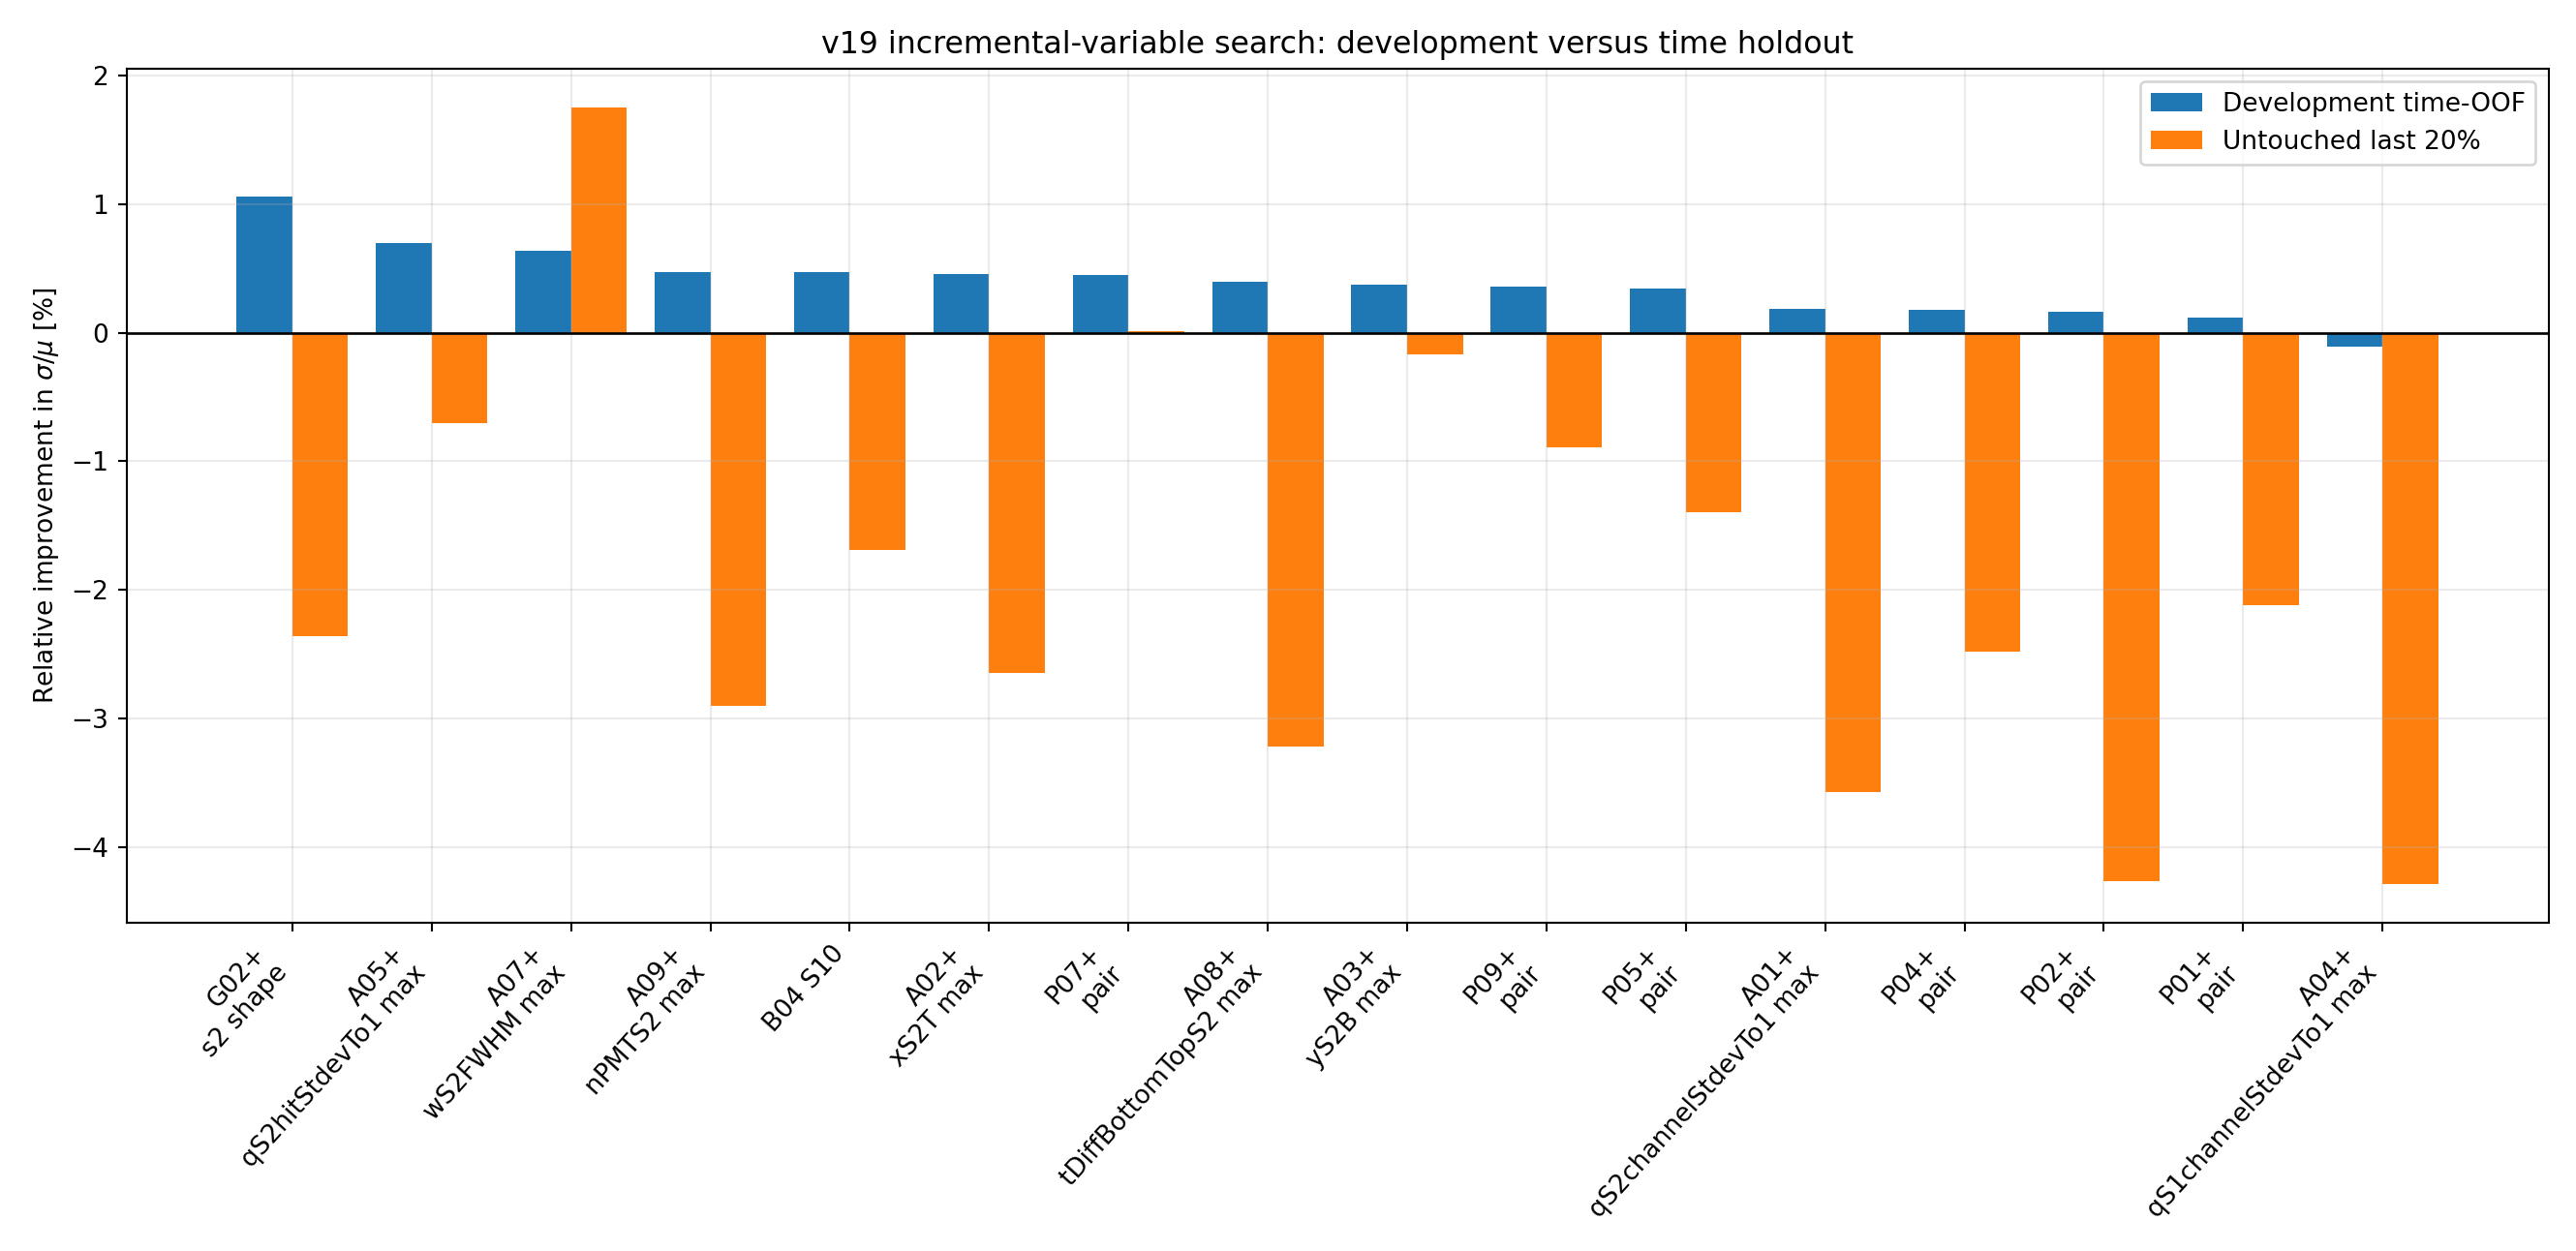
\includegraphics[width=0.94\linewidth,height=0.72\textheight,keepaspectratio]{01_feature_set_comparison.png}
\smallnote{蓝色为前 80\% 时间段的 OOF 改善；橙色为最后 20\% 完全留出段。负值表示变差。}
\end{frame}

\begin{frame}{5. 逐个增加变量的消融结果}
\centering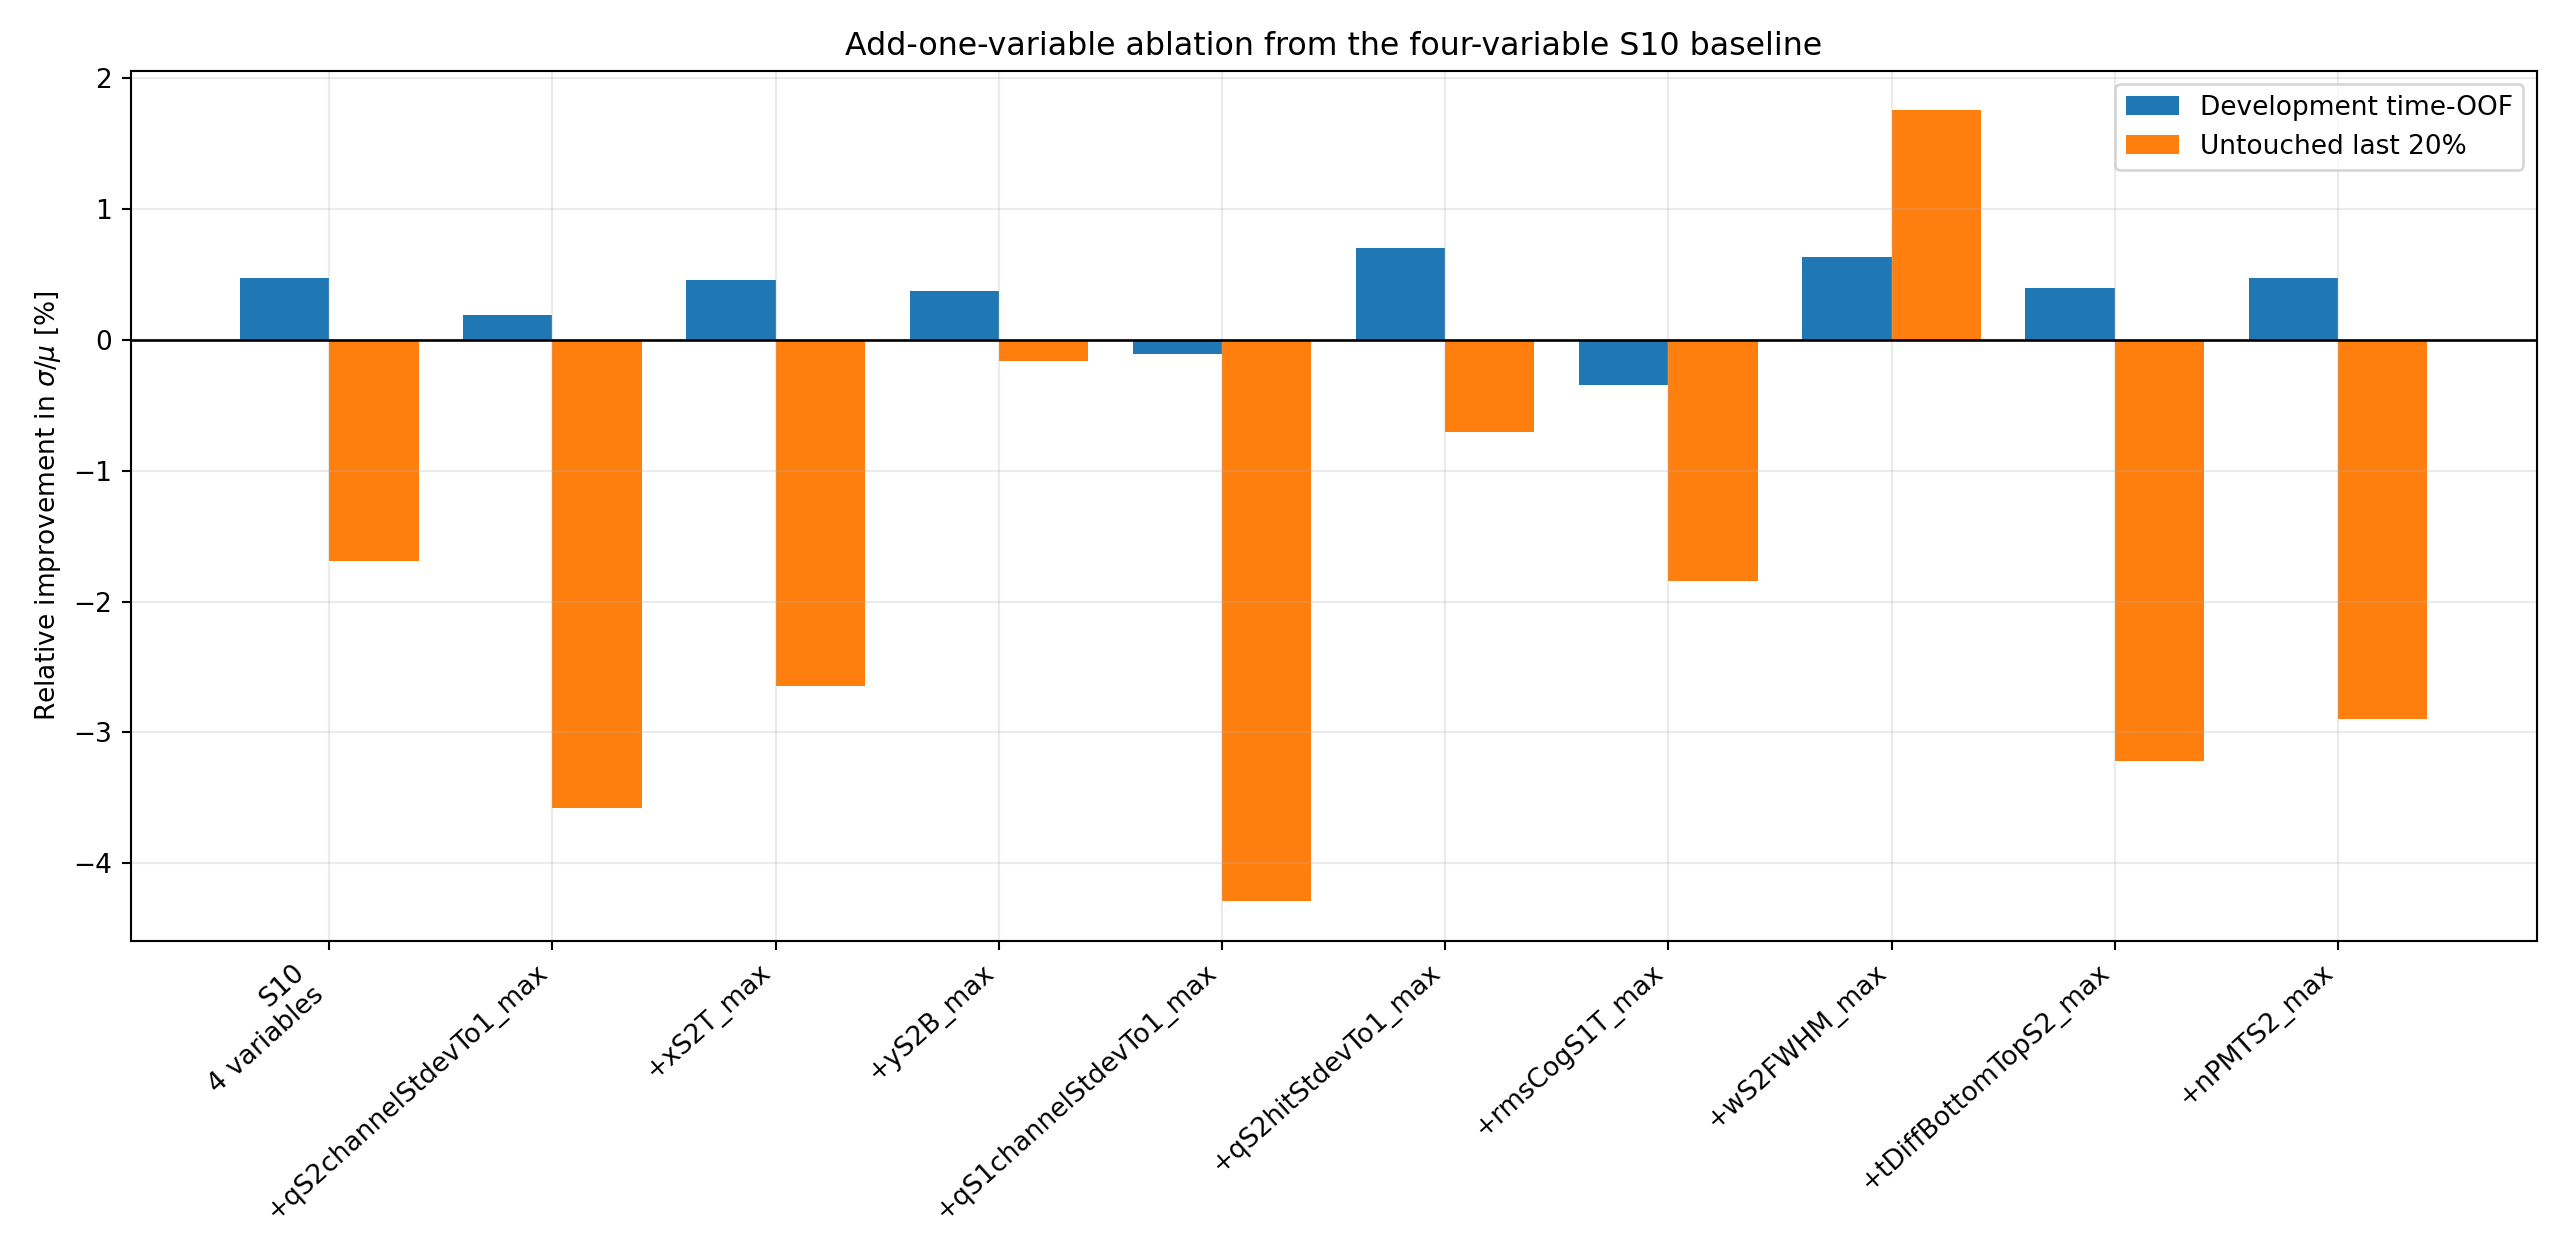
\includegraphics[width=0.94\linewidth,height=0.72\textheight,keepaspectratio]{02_single_variable_ablation.png}
\smallnote{多数变量在开发段呈现小幅正收益，但在独立时间段发生反转，说明存在明显时间依赖。}
\end{frame}

\begin{frame}{6. 三个指标必须一起看}
\centering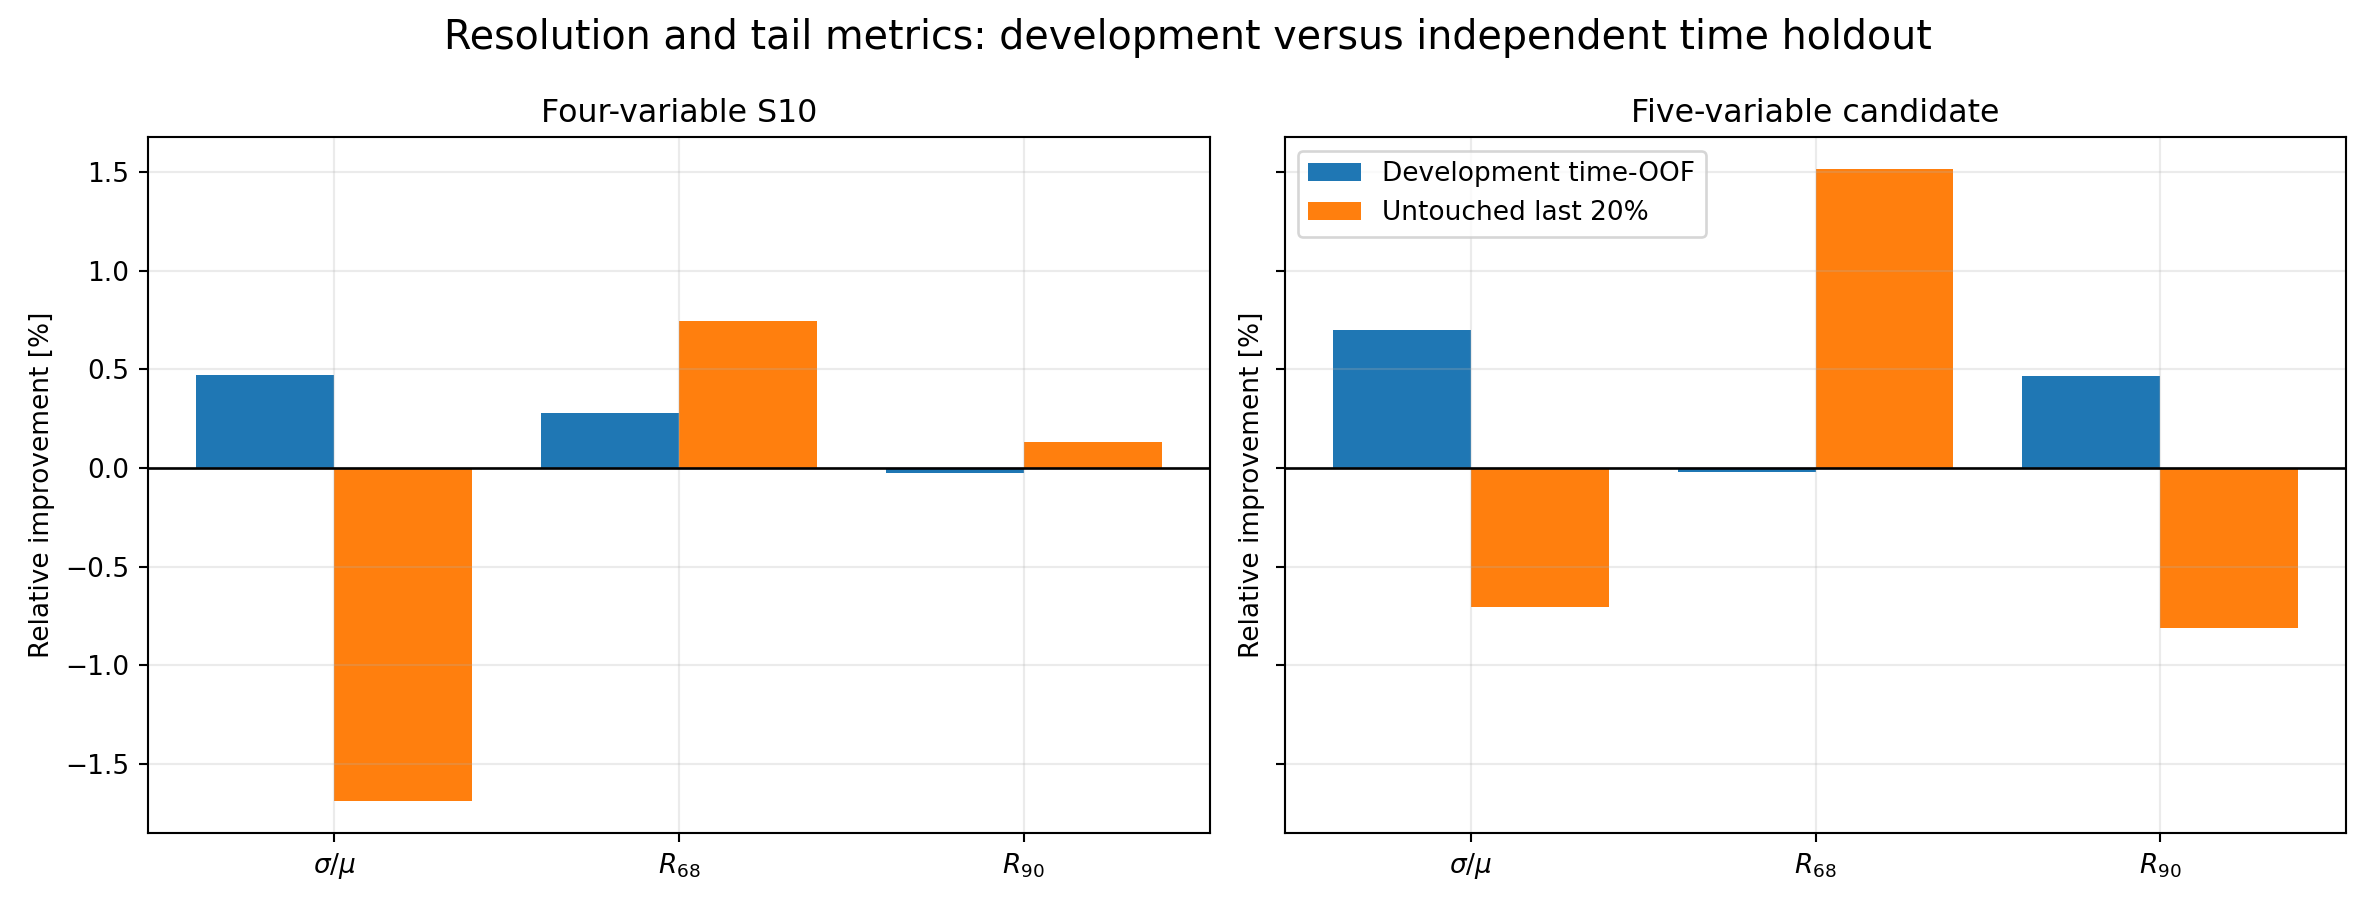
\includegraphics[width=0.91\linewidth,height=0.74\textheight,keepaspectratio]{08_metric_summary.png}
\smallnote{五变量候选加入 $qS2hitStdevTo1_{\max}$；留出段的 $\sigma/\mu$ 与 $R_{90}$ 均变差。}
\end{frame}

\begin{frame}{7. 五变量候选为什么被否决}
\begin{columns}[T,onlytextwidth]\column{0.48\textwidth}
\begin{block}{开发段选出的候选}
\[\begin{aligned}\mathbf{x}=\{&dt,\;wS2CDF_{\max},\;yS2Tcor_{\max},\\&xS2Bcor_{\max},\;qS2hitStdevTo1_{\max}\}.\end{aligned}\]
$\alpha=300$，最大对数修正为 0.0075。
\end{block}
\column{0.49\textwidth}\small
\begin{tabular}{lcc}\toprule 指标 & 开发段 & 最后 20\%\\\midrule
$\sigma/\mu$ 改善 & \good{+0.700\%} & \warn{$-0.706\%$}\\
$R_{68}$ 改善 & $-0.022\%$ & \good{+1.514\%}\\
$R_{90}$ 改善 & \good{+0.465\%} & \warn{$-0.813\%$}\\\bottomrule\end{tabular}
\vspace{0.35cm}\begin{block}{判定}候选未通过独立时间验证，不能替代四变量模型。\end{block}
\end{columns}
\vspace{0.25cm}\centering\warn{结论：本轮没有确认“变量越多越好”。}
\end{frame}

\begin{frame}{8. 标定与本底能谱的直接对比}
\centering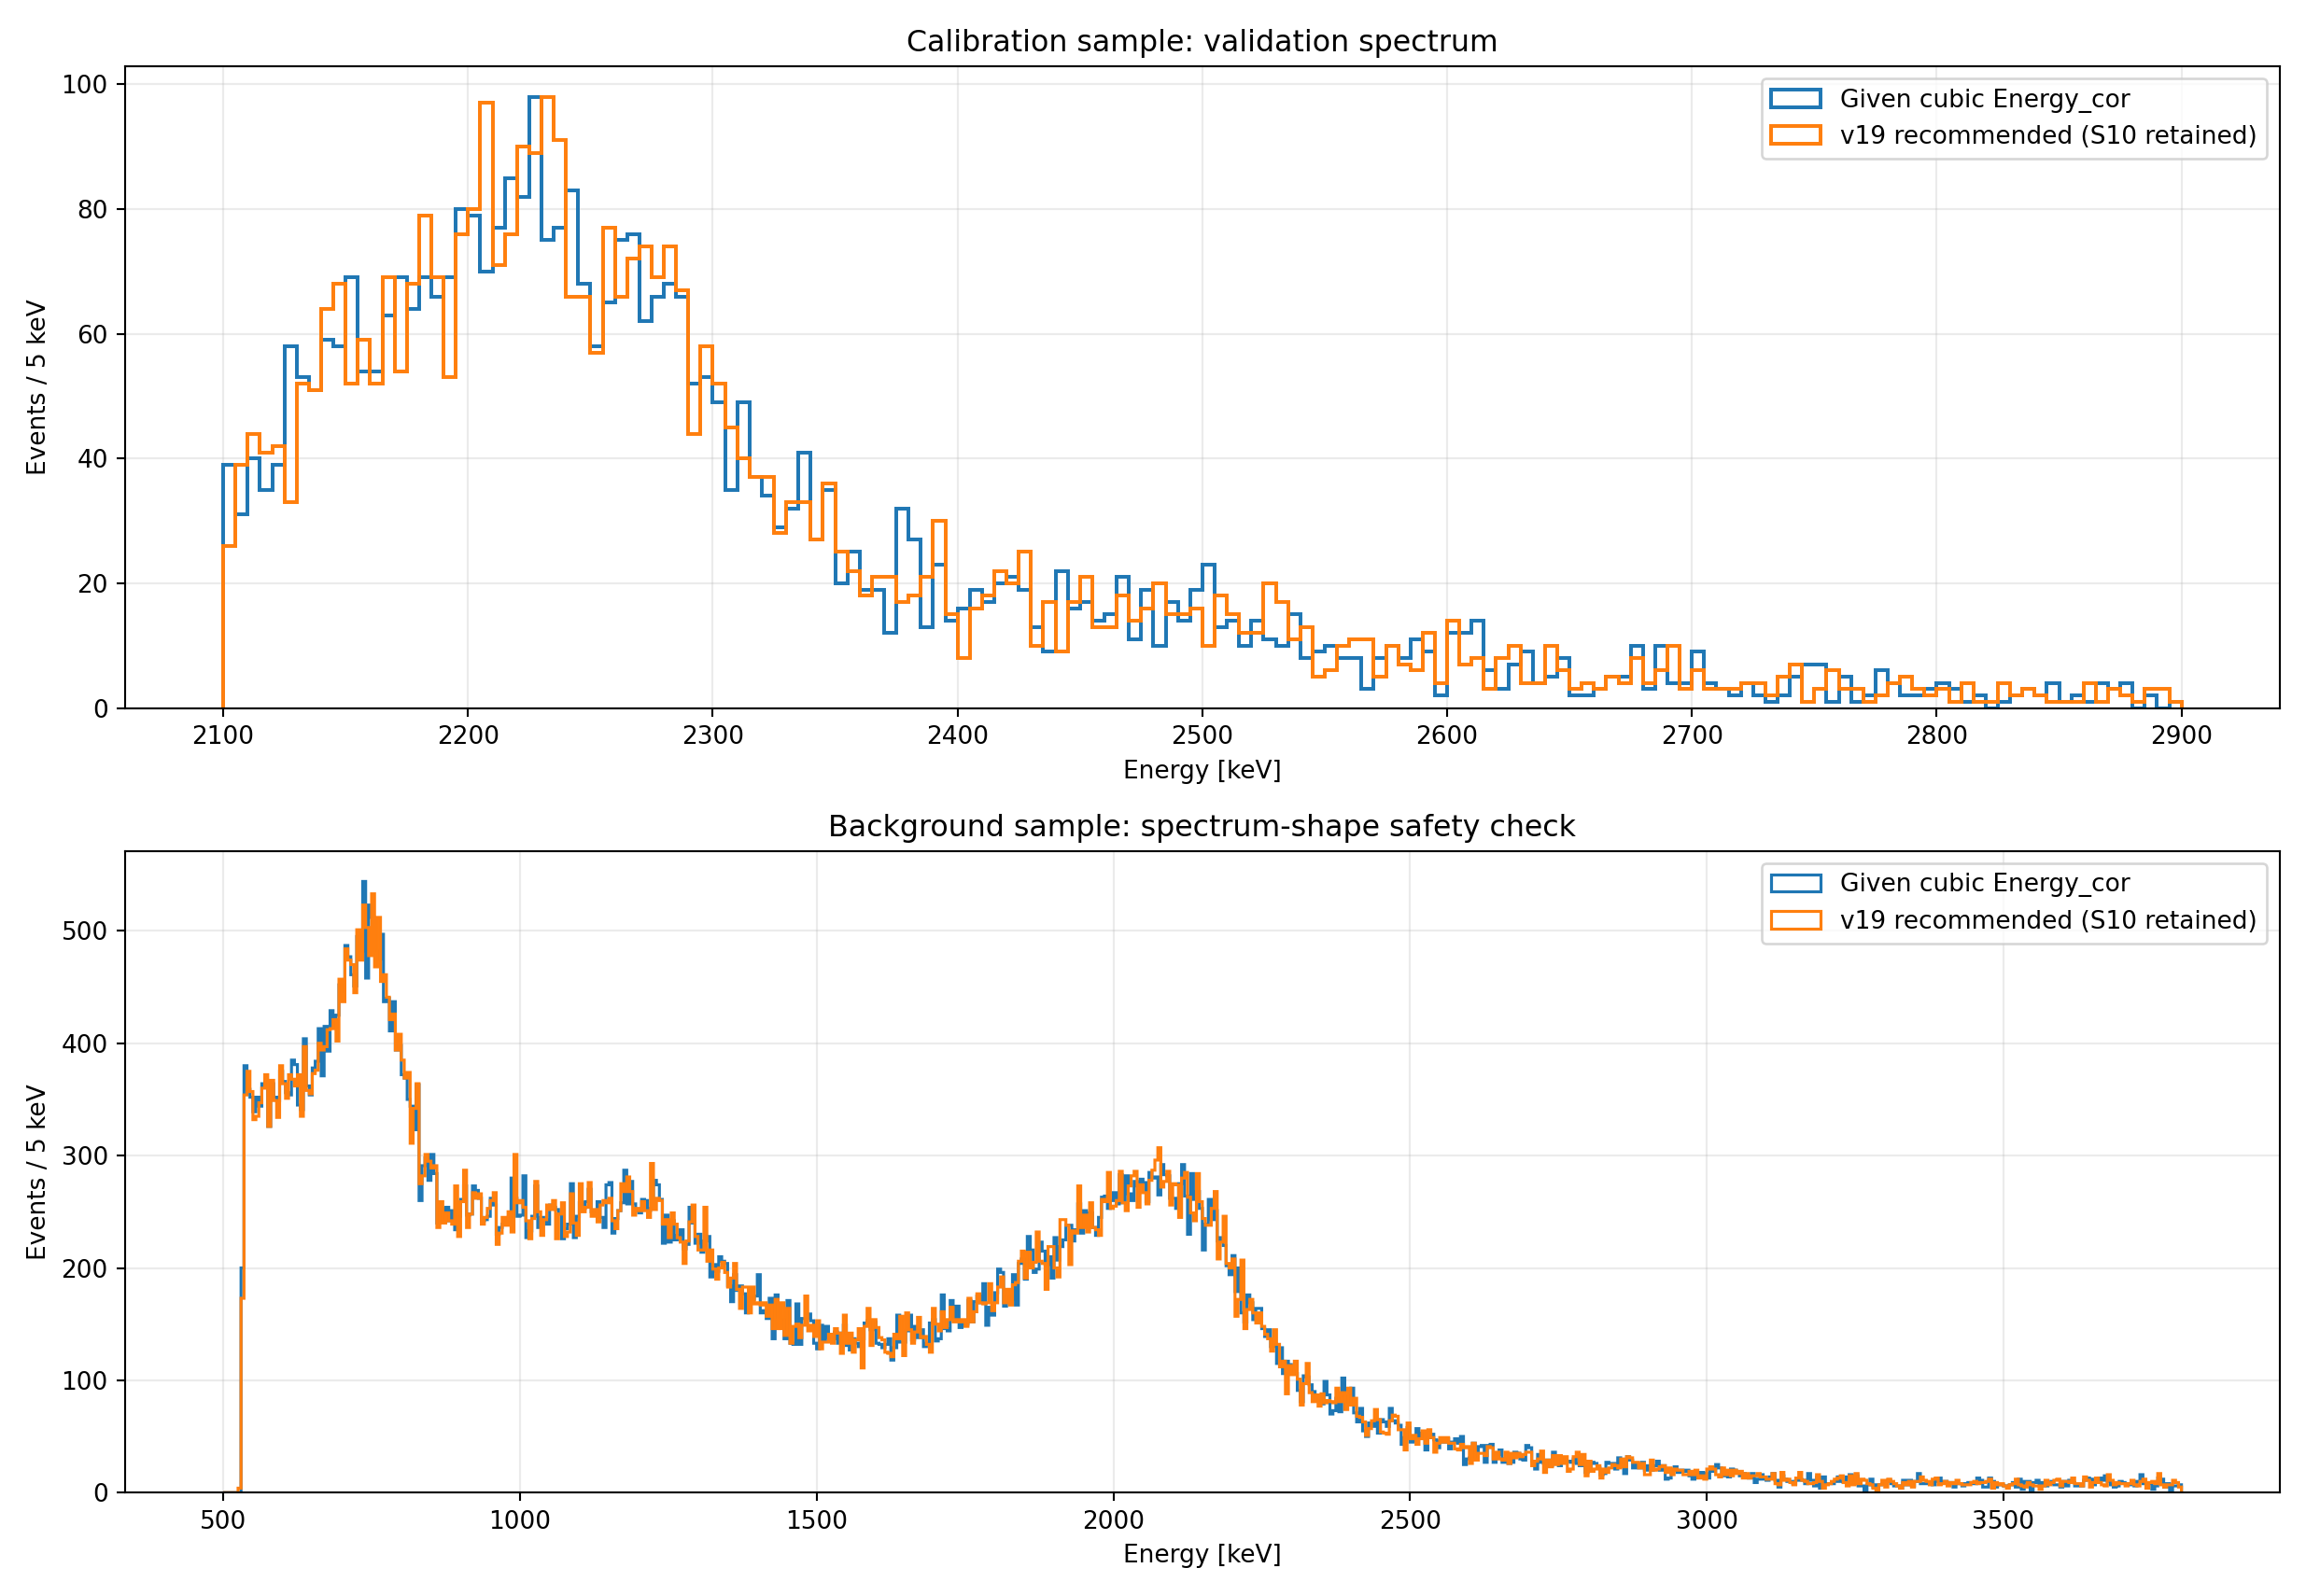
\includegraphics[width=0.91\linewidth,height=0.72\textheight,keepaspectratio]{03_energy_spectra.png}
\smallnote{蓝色为给定三次能量，橙色为 v19 最终保留输出；v19 仍采用四变量方案。}
\end{frame}

\begin{frame}{9. 2450--3000 keV：假峰安全检查}
\centering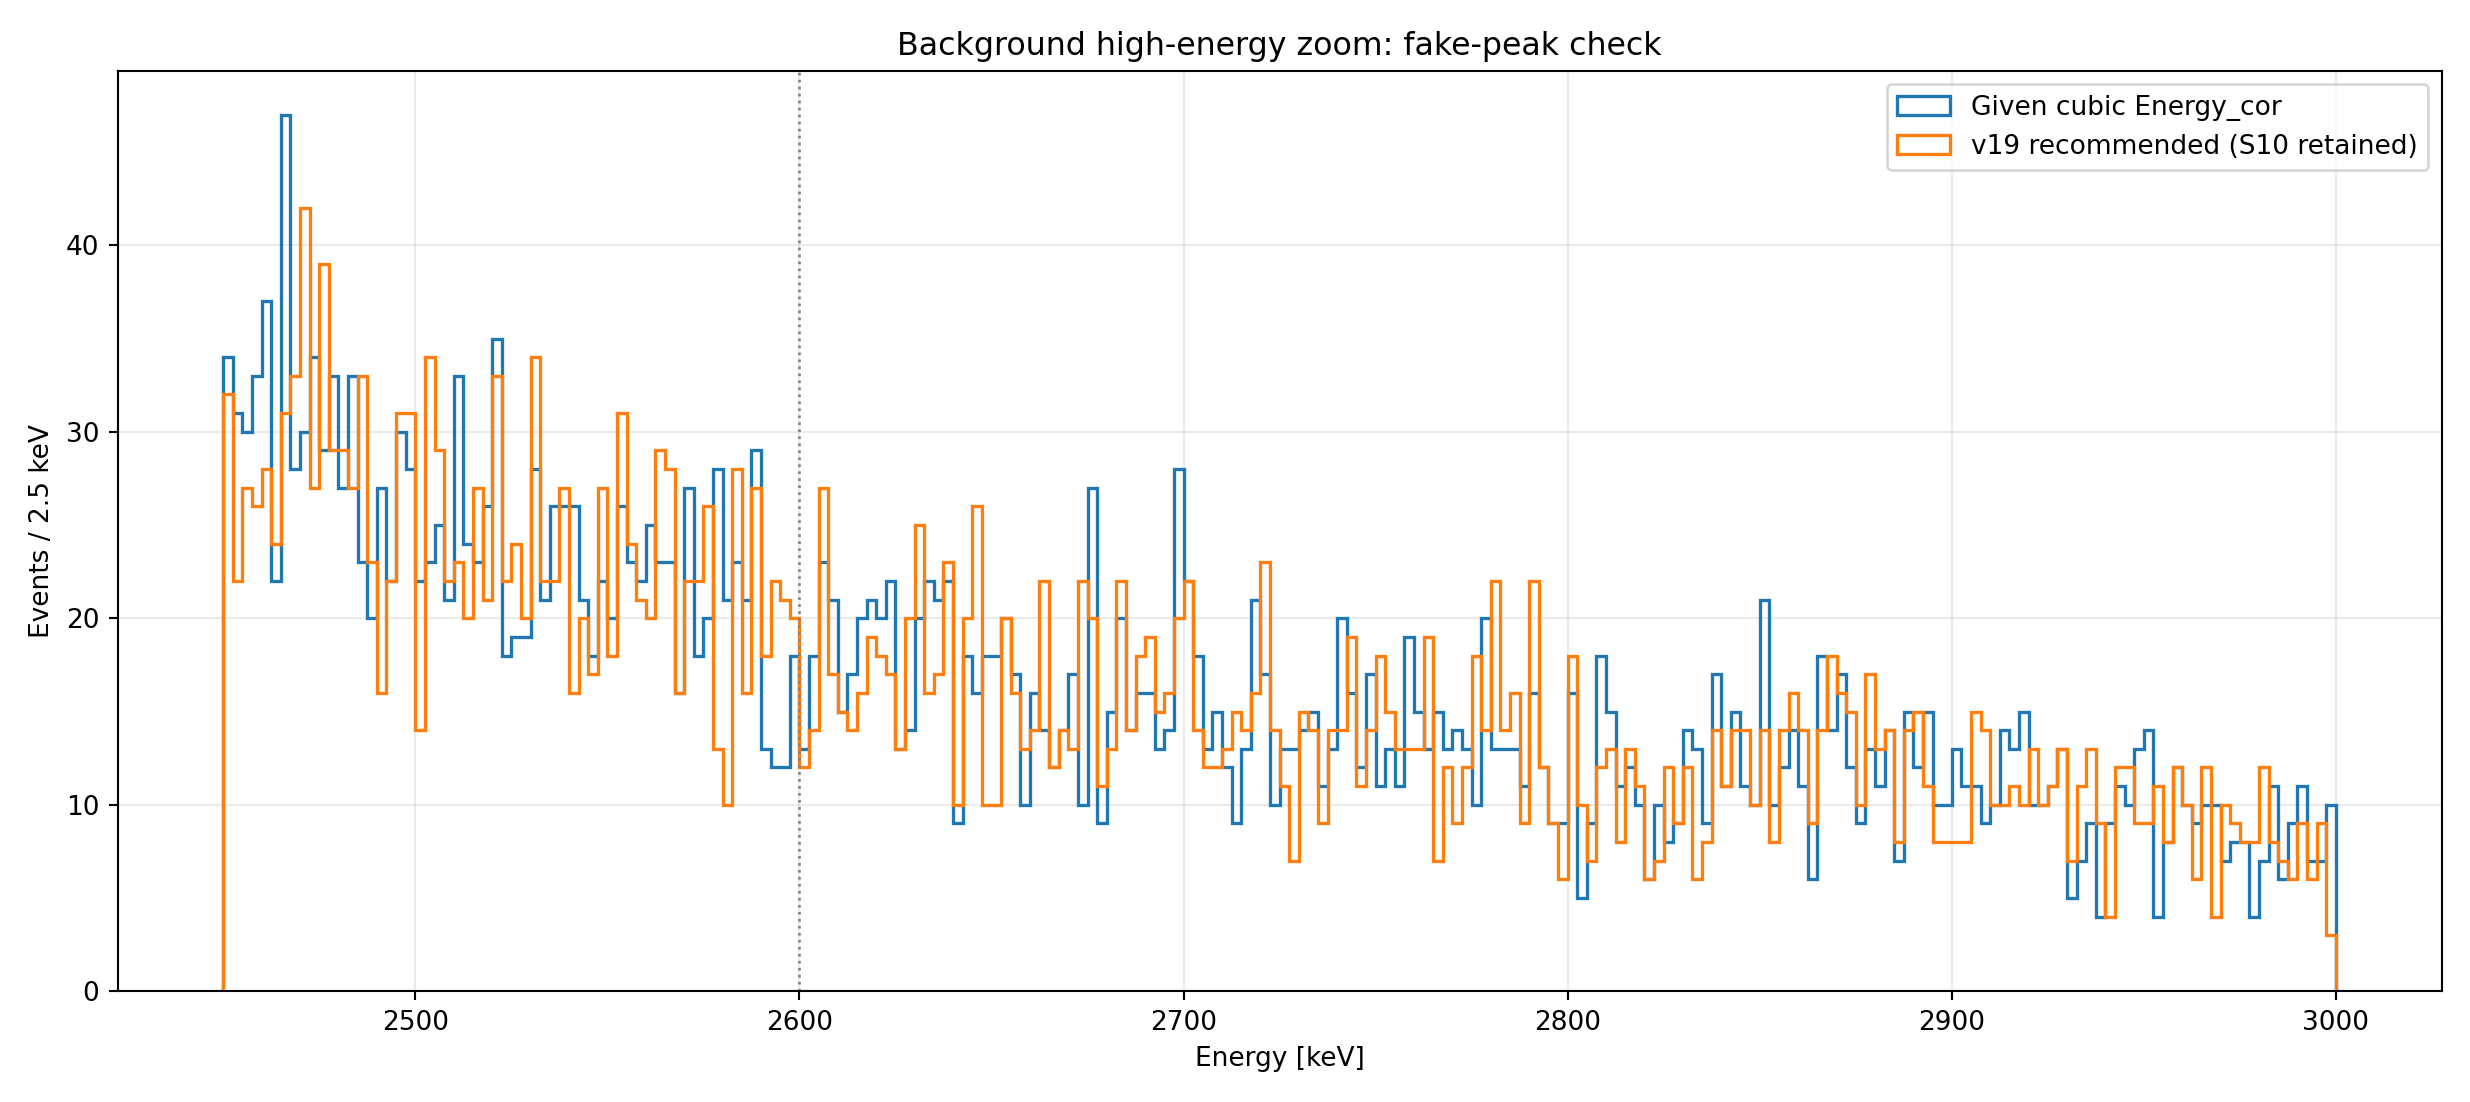
\includegraphics[width=0.93\linewidth,height=0.76\textheight,keepaspectratio]{05_background_2450_3000_zoom.png}
\smallnote{虚线标出 2600 keV。两条曲线只出现统计涨落，没有重新形成异常窄峰。}
\end{frame}

\begin{frame}{10. 标定样本：修正比值与四个输入量}
\centering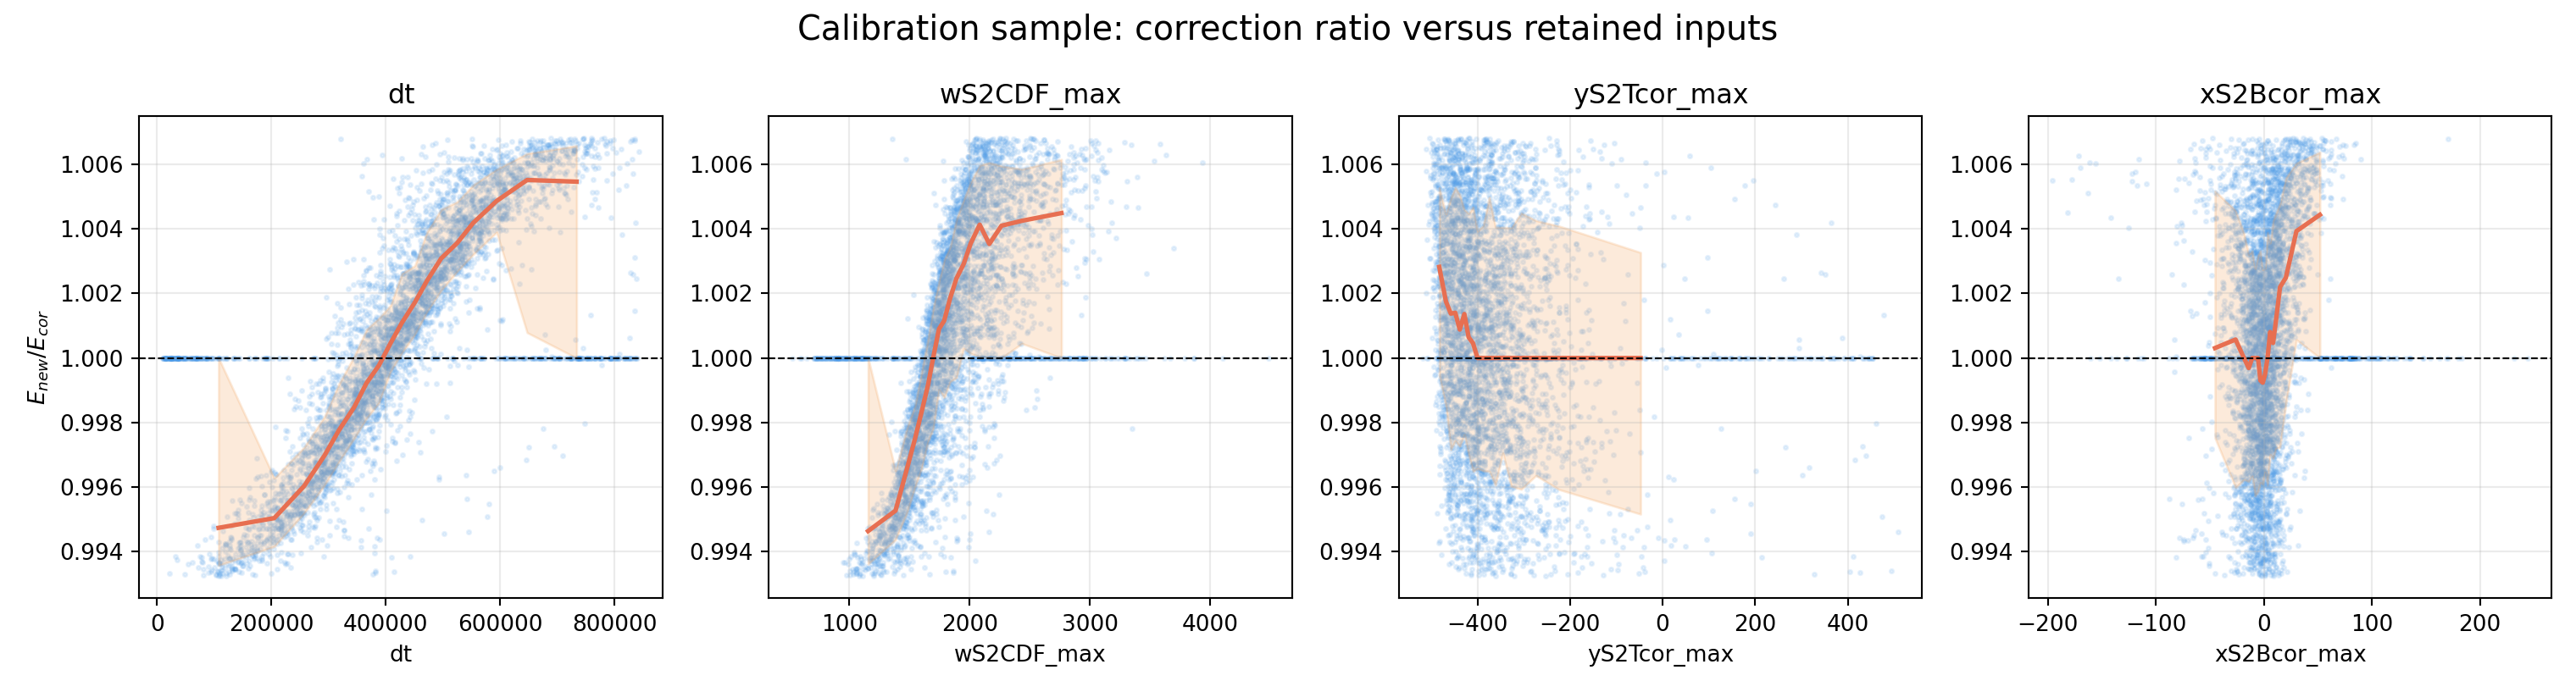
\includegraphics[width=0.96\linewidth,height=0.74\textheight,keepaspectratio]{06_calibration_ratio_vs_inputs.png}
\smallnote{橙线为分箱中位数，橙色区域为 16\%--84\% 区间；$dt$ 和 S2 宽度仍是主要变化方向。}
\end{frame}

\begin{frame}{11. 本底样本：相同趋势明显减弱}
\centering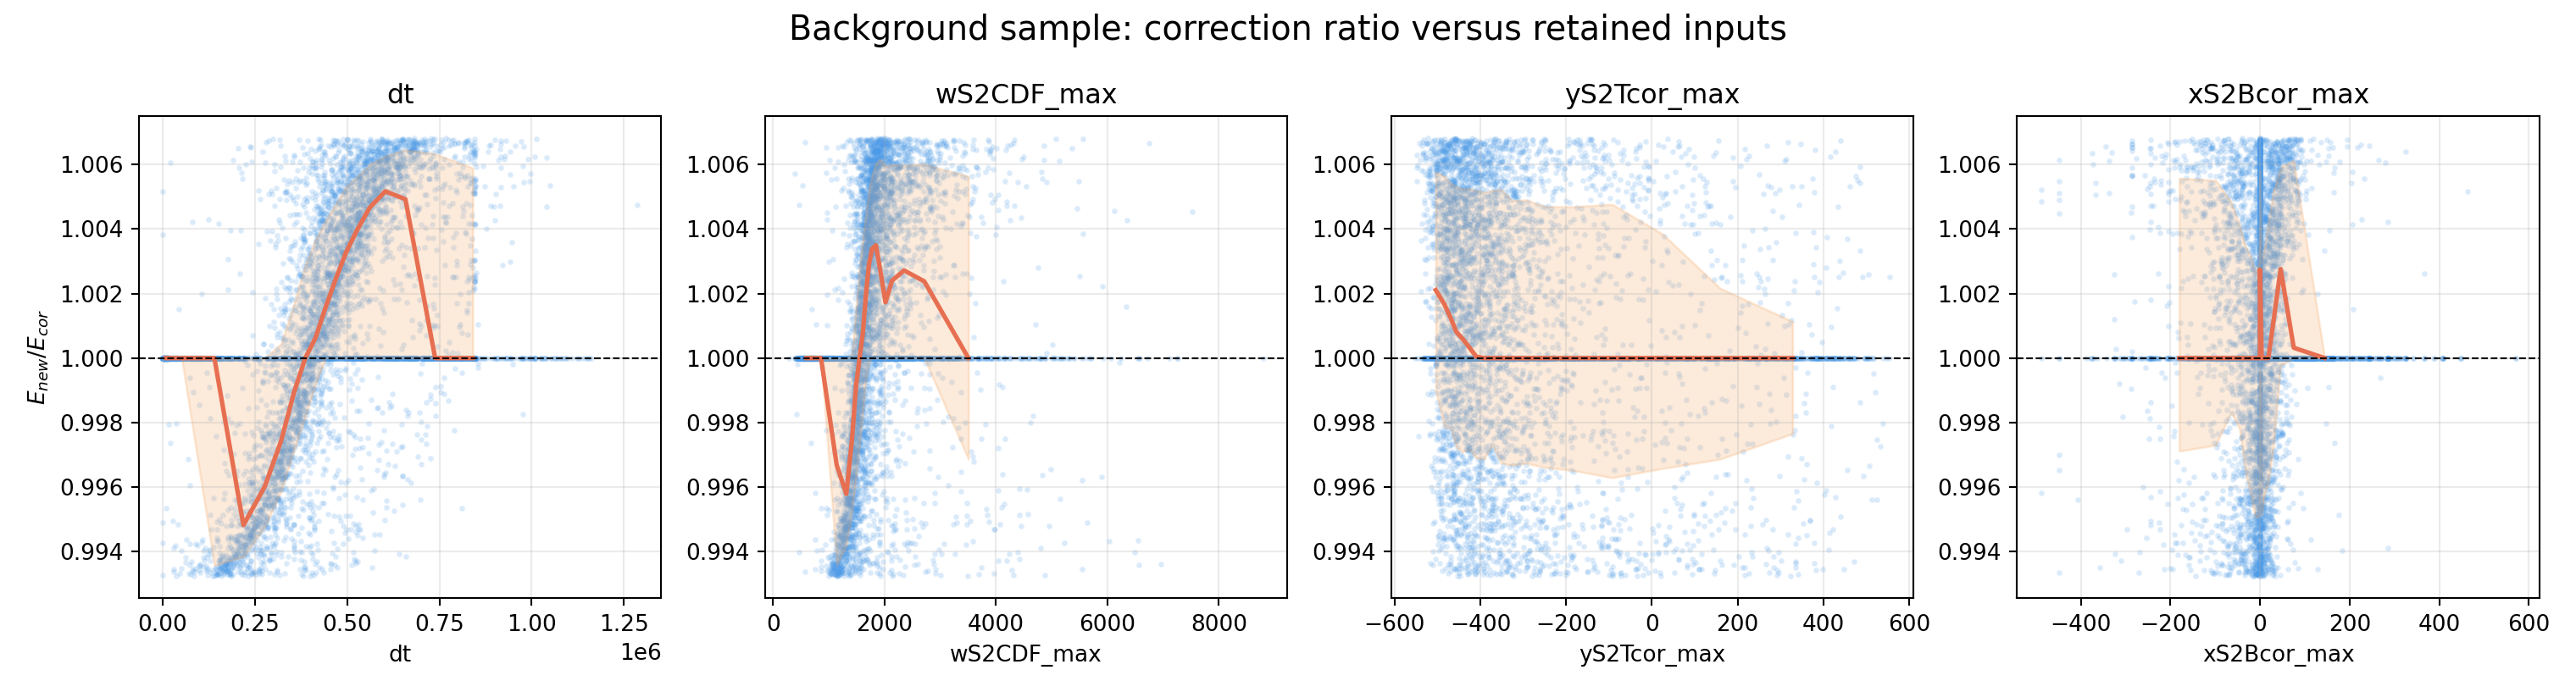
\includegraphics[width=0.96\linewidth,height=0.74\textheight,keepaspectratio]{07_background_ratio_vs_inputs.png}
\smallnote{大量本底事件保持 $E_{\rm new}/E_{\rm cor}=1$；位置变量只提供小幅细化。}
\end{frame}

\begin{frame}{12. 按时间分块检查修正稳定性}
\centering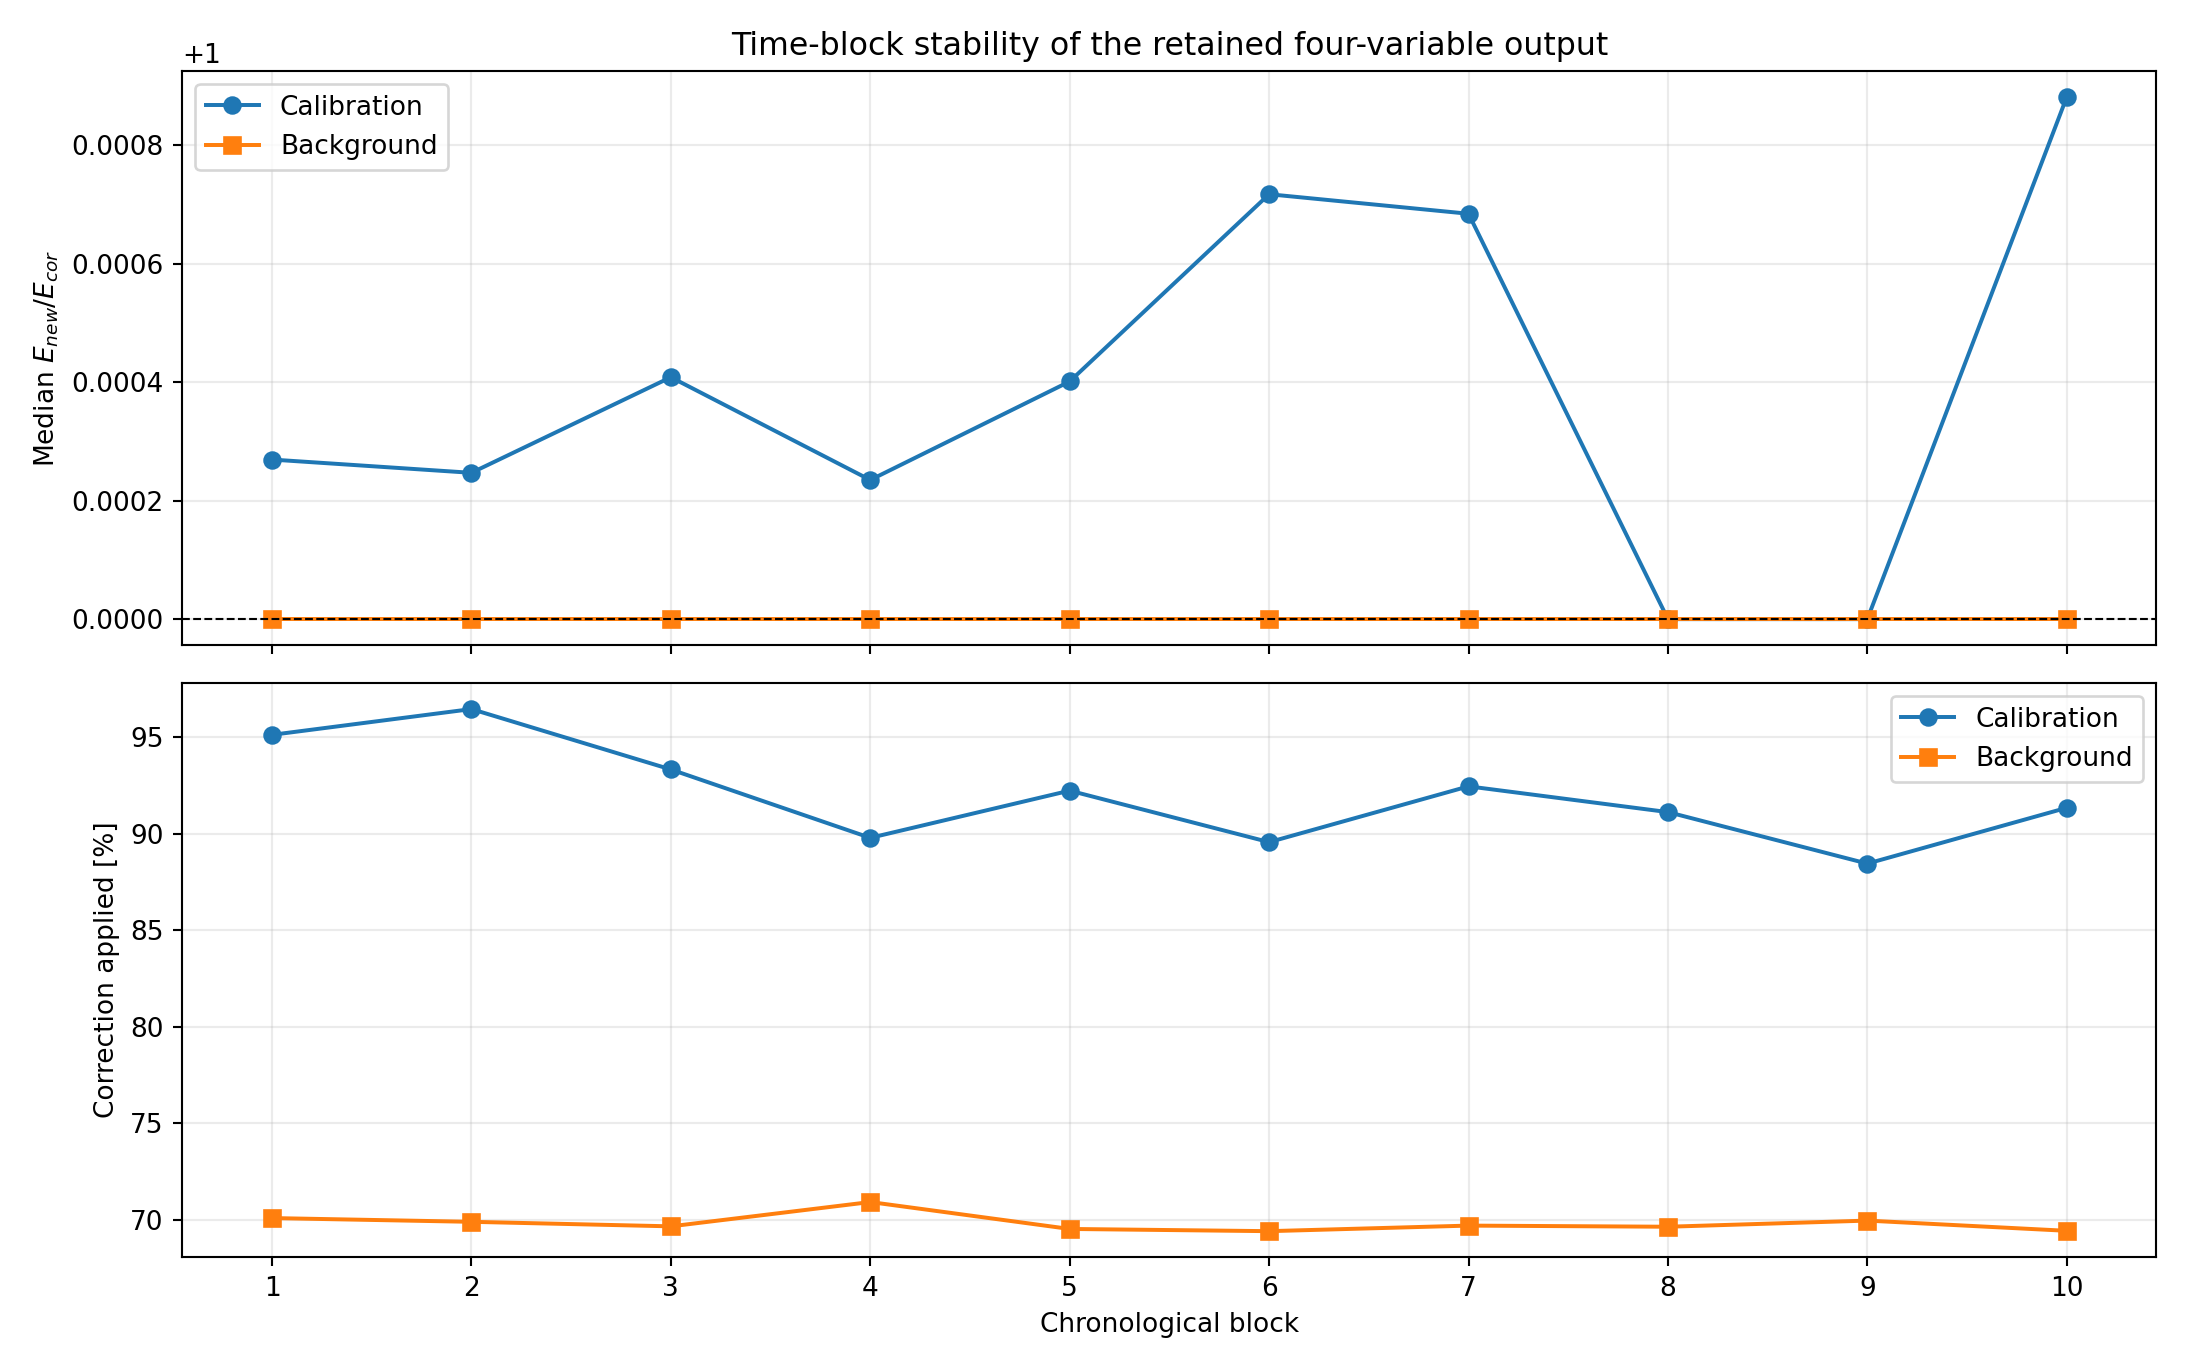
\includegraphics[width=0.89\linewidth,height=0.74\textheight,keepaspectratio]{09_time_block_stability.png}
\smallnote{上图为中位修正比，下图为执行修正的事件比例；标定段仍显示时间变化。}
\end{frame}

\begin{frame}{13. 当前能够成立的结论}
\begin{columns}[T,onlytextwidth]\column{0.48\textwidth}
\begin{block}{本轮已经完成}\begin{itemize}\item 训练并筛选 288 个候选；\item 测试 9 个新增物理变量；\item 加入独立时间留出验证；\item 完成本底全谱与 2600 keV 检查；\item 生成输入关系图和时间稳定性图。\end{itemize}\end{block}
\column{0.49\textwidth}
\begin{block}{当前模型状态}\begin{itemize}\item 新增变量没有通过最终验证；\item 暂时保留四变量输出；\item 四变量模型也不是最终物理模型；\item 主要限制已转向时间漂移和单 run 泛化。\end{itemize}\end{block}
\end{columns}
\vspace{0.3cm}\centering\Large\color{navy}\bfseries 下一步应优先加入新 run 和多能量峰，\\而不是继续无约束增加变量。
\end{frame}
\end{document}
